\documentclass{article}

% Language setting
% Replace `english' with e.g. `spanish' to change the document language
\usepackage[spanish]{babel}

% Set page size and margins
% Replace `letterpaper' with `a4paper' for UK/EU standard size
\usepackage[a4paper,top=2.5cm,bottom=2.5cm,left=3.5cm,right=3.5cm,marginparwidth=2.5cm]{geometry}

% Useful packages
\usepackage{amsmath}
\usepackage{graphicx}
\usepackage[gen]{eurosym}
\usepackage{siunitx}
%Podemos cambiar el color del Índice(negro), los enlaces están marcados en azul. 
\usepackage[colorlinks=true, linkcolor=black, urlcolor=blue]{hyperref}
\usepackage{fancybox}
\usepackage{listings}
\usepackage{subcaption}
%\lstset{
%    language=Matlab,
%    extendedchars=true
%}

\title{Diseño de Redes Inalámbricas en La Costera}
\author{Andé Yermak y Álvaro Hernández}
%\date{}

\begin{document}
\maketitle

%Aquí se generará nuestro Índice, podemos poner /newpage para tenerlo solo en la página
\tableofcontents
\newpage

\section{Introducción}

Se pretende dotar de acceso a internet a determinadas zonas de La Costera, Murcia. Una pedanía situada cerca de Alhama donde residen alrededor de 400 habitantes. La idea planteada será personalizar, según la necesidad, cada una de las zonas propuestas para su funcionamiento, y a su vez reducir al máximo el coste de instalación.

\begin{figure}[ht]
    \centering
    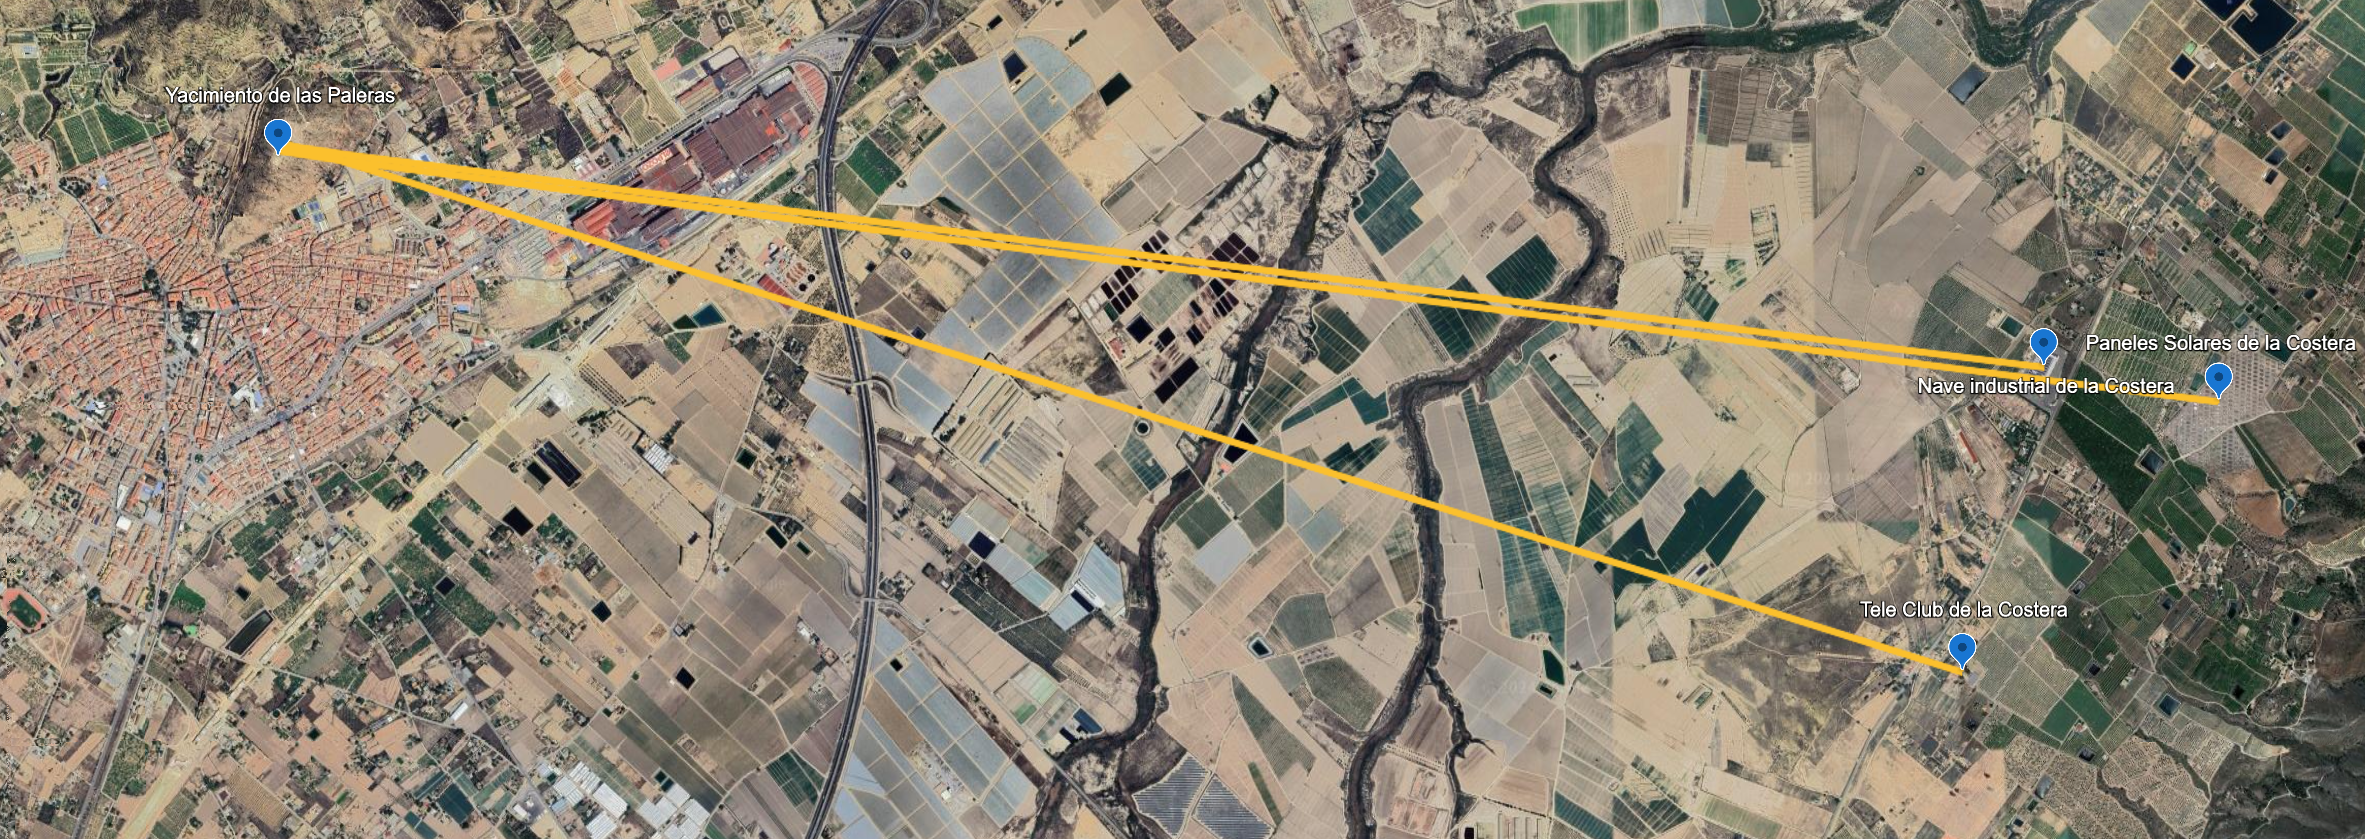
\includegraphics[width=0.8
    \linewidth]{src/earthpoints.png}
    \caption{\label{fig:earthpoints} Mapa de los puntos de radio enlace.}
\end{figure}

\quad

Al ser un servicio propuesto por el ayuntamiento, se usarán bandas de frecuencia de la red troncal, es decir, de $5GHz$ y de $2.4GHz$, donde no será necesario cierta cantidad de trámites para usarlas a comparación de otras personalizadas, además de ser gratis el añadido de radioenlaces. Por otro lado, se limitarán ciertos parámetros como la potencia de transmisión.

\subsection{Planteamiento de TeleClub}

El teleclub es un centro social que necesita de internet tanto \textbf{indoor} como \textbf{outdoor}. De puertas para dentro estará la biblioteca, lugar donde la conexión es de suma importancia para tareas como descarga de ebooks o registros en su web de usuarios. En el exterior del teleclub, se dotará de internet básico para el ocio que puedan tener los visitantes y residentes, se tiene en cuenta que el exterior tendrá un mayor número de usuarios.

\quad

\begin{figure}[ht]
    \centering
    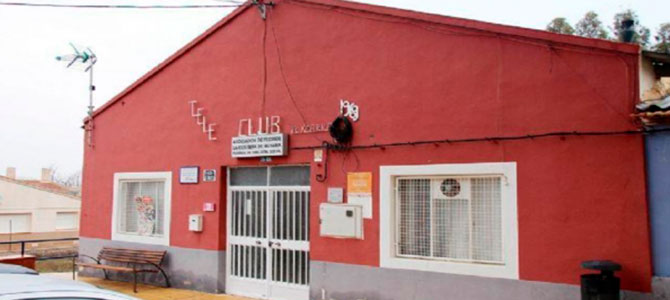
\includegraphics[width=0.5\linewidth]{src/teleclub.jpg}
    \caption{\label{fig:teleclub} Fachada del TeleClub.}
\end{figure}


Según la población de \textbf{La Costera}, que es de 343 habitantes, (Actualizado febrero 2023), se puede considerar que el tráfico de TeleClub no superará el 20\% de la población total. Ésto es de aproximadamente 75 usuarios. Se añadirá un margen debido al turismo de 25 usuarios, por lo que el máximo tráfico cursado será de \textbf{100 usuarios}.

\quad

Para calcular el \textbf{throughput} que consumirá nuestra sección del TeleClub, se planteará el concepto de \textbf{usuario típico}, que se multiplicará por la cantidad de éstos. Se denominará a aquél que utiliza el correo, navega por Internet y ocasionalmente transmite/recibe ficheros de gran tamaño. A día de hoy, la mayor velocidad necesitada para este tipo de tareas será de \textbf{1Mbps}

    $$100u \cdot 1Mbps = 100Mbps$$

El throughput para esta zona será de \textbf{100Mbps}.

\subsection{Planteamiento de la Nave}

En la Nave habrá un máximo de 30 usuarios, que debido a los servidores web y redes necesitan de 10Mbps como máximo en total, por lo que definirá el throughput de esta sección. (añadir 4 AP)

\subsection{Planteamiento de Paneles}

\textbf{EXPLICAR REPARTO CAMARAS ETC}
\begin{figure}[ht]
    \centering
    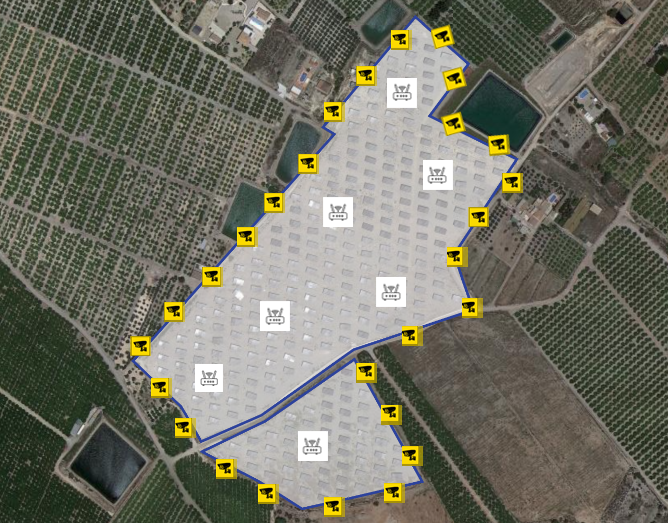
\includegraphics[width=0.4\linewidth]{src/camaras.png}
    \caption{\label{fig:camarasnave} Reparto de las cámaras y access points.}
\end{figure}



28 cámaras por 1Mbps
$$28u \cdot 10Mbps$$

\section{Materiales elegidos}

\subsection{Materiales comunes}
Los switches se eligirán unos económicos de una marca confiable, puesto que el uso que se hará en un pueblo de pocos habitantes será mucho menor a otros que requieren de tecnología más sofisticada. Éstos switches suelen tener vida útil limitada, pero es con respecto a la garantía, no significa que su uso esté limitado a cierto tiempo:

\quad

Para los switches que requieran 8 puertos o menos se usará el \textbf{Switch TL-SG108E Easy Smart de 8 puertos Gigabit}, de la marca TP-link. Se trata de un switch no gestionado y económico, diseñado para pequeñas y medianas empresas que requieren de redes con gestión simple. Para optimizar el tráfico en su red de negocios, el switch ofrece QoS basado en puerto y en etiquetas para mantener el tráfico sensible a la latencia sin problemas y sin fluctuaciones. Además, el gasto energético no será elevado, puesto que el TL-SG108E puede ahorrar hasta un 80\% del consumo de energía, lo cual es una solución ecológica para su red de negocios. 

Para la nave, donde hará falta uno de más puertos, se usará el \textbf{TP-Link TL-SF1016DS de 16 puertos.} Ya que el modelo anterior no tiene opción de más puertos, este sería su equivalente. 

\begin{figure}[h]
	\centering
	\begin{subfigure}{0.3\textwidth}
		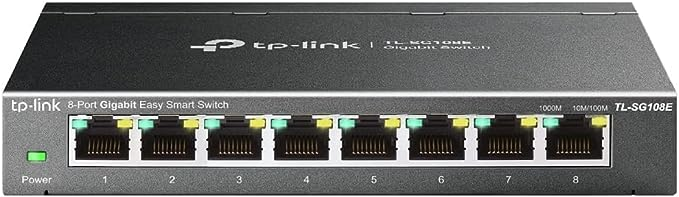
\includegraphics[width=\linewidth]{src/switch 8.jpg}
		\caption{Switch de 8 Puertos}
		\label{fig:switch8}
	\end{subfigure}%
	\begin{subfigure}{0.3\textwidth}
		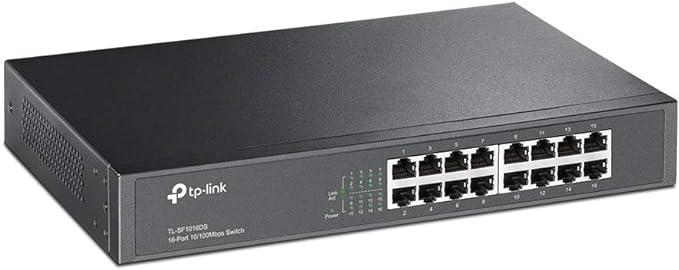
\includegraphics[width=\linewidth]{src/switch 16.jpg}
		\caption{Switch de 16 Puertos}
		\label{fig:switch16}
	\end{subfigure}
	\caption{}
	\label{fig:switches}
\end{figure}

Los access points serán de la marca \textbf{Ubiquiti}, al igual que las antenas usadas. En este caso, el \textbf{Ubiquiti Networks UAP-AC-LR}. Según su \href{https://dl.ubnt.com/datasheets/unifi/UniFi_AC_APs_DS.pdf}{Datasheet}, tiene soporte para VLANs, protocolos de privacidad y seguridad como \textbf{WPA2}, y compatibilidad con las antenas Ubiquiti elegidas.

\quad

Se usará una estación base Ubiquiti Rocket R2AC-PRISM al ser la que mejor cumple las necesidades con un coste reducido, al igual que una compatibilidad con las antenas \textbf{Ubiquiti}. De tal modo que se podrá crear un ecosistema de la misma marca en distintos puntos con compatibilidad y fácil asistencia. Según su \href{https://dl.ubnt.com/datasheets/RocketAC/Rocket_R2AC_DS.pdf}{Datasheet}, consigue un SNR elevado, y trabaja solo en frecuencias de $2.4GHz$, de este modo se consigue una reducción del precio al no usarse en ningún momento bandas de frecuencia de $5GHz$.

\begin{figure}[ht]
	\centering
	\begin{subfigure}{0.4\textwidth}
		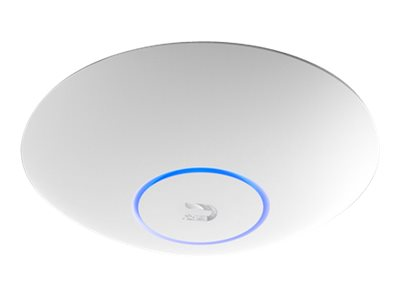
\includegraphics[width=\linewidth]{src/ap.jpg}
		\caption{Access Point Ubiquiti}
		\label{fig:ap}
	\end{subfigure}%
	\begin{subfigure}{0.3\textwidth}
		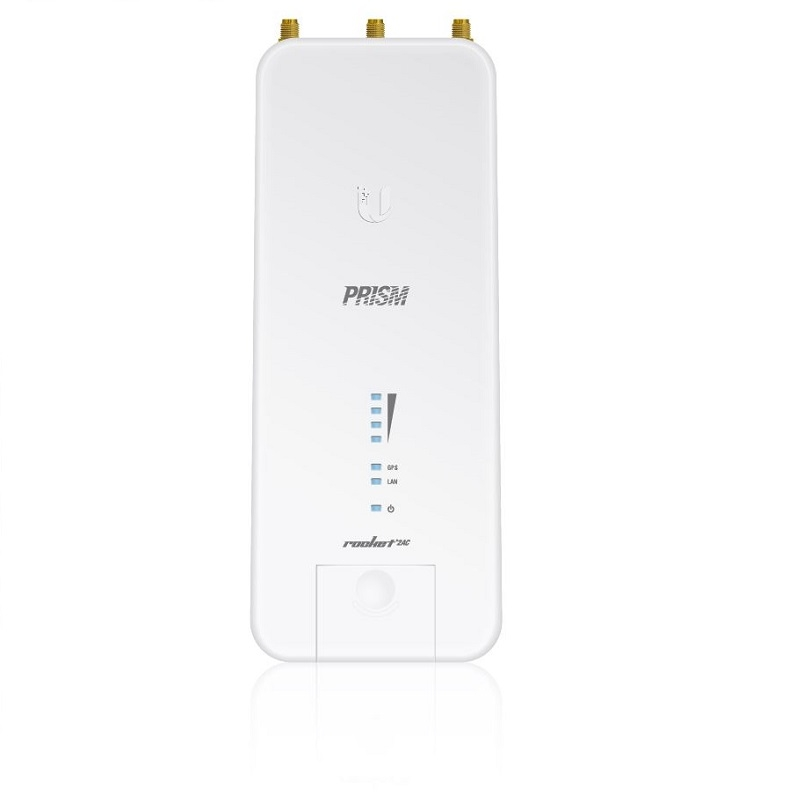
\includegraphics[width=\linewidth]{src/estacion base.jpeg}
		\caption{Estación Base}
		\label{fig:estacionbase}
	\end{subfigure}
	\caption{}
	\label{fig:accesspoint}
\end{figure}
\subsection{Radioenlaces}

Se ha proporcionado en el aula virtual un \href{http://www.microcom.com.ar/fotos/ficha7097LBE-M5-23.compressed.pdf}{Datasheet} donde aprovecharemos para elegir el material que más se adapte a nuestros planteamientos. 

\quad

Se usará de antena transmisora el Ubiquiti LBE-5AC-16-120, ya que al ser omnidireccional permite transmitir en distintas direcciones. Dicha antena se situará en Alhama, específicamente en el Yacimiento de las Paleras, por tener mayor elevación respecto al resto de la zona para una transmision mejor. Junto a esta antena, se conectará la estación base Rocket Prism R2AC.

\quad

En las otras tres ubicaciones, situadas en la \textbf{Nave}, \textbf{TeleClub}, y los \textbf{paneles}, se usarán antenas unidireccionales pusto que su única conexión será con la antena transmisora. En el \textbf{Datasheet proporcionado}, la antena que cumple con los requisitos es la Ubiquiti LBE-5AC-23.

\subsection{TeleClub}

En el TeleClub, se recibe la señal principal en la antena LBE-5AC-23, y se repartirá la conexión mediante un switch a dos Access Points: que servirán para \textbf{Indoor} y \textbf{Outdoor}.    


\subsection{Nave}
\subsection{Paneles}

\section{Presupuesto}

\begin{table}[h]
    \centering
    \begin{tabular}{|c|c|c|c|}
        \hline
        Material & Cantidad & Precio & Suma\\
        \hline
        Switch TL-SG108E & 2 & $31.99\euro{}$ & $63.98\euro{}$\\
        Switch TL-SF1016DS & 1 & $59.69\euro{}$ & $119.38\euro{}$ \\
        Ubiquiti LBE-5AC-16-120  & 1 & $102.58\euro{}$ & $102.58\euro{}$\\
        Ubiquiti LBE-5AC-23& 2 & $73.89\euro{}$ & $147.78\euro{}$ \\
        E. Base R2AC-PRISM & 1 & $207.50\euro{}$ & $207.50\euro{}$ \\
        \hline
        Total &  &  & $581.53\euro{}$ \\

        \hline
    \end{tabular}
    \caption{Tabla del presupuesto total}
    \label{tab:presupuestos}
\end{table}
\newpage


\section{Normativa PIRE}

La banda de frecuencias 2400-2483,5 MHz, designada en el Reglamento de
Radiocomunicaciones para aplicaciones industriales, científicas y médicas (ICM),
podrá ser utilizada también para los siguientes usos de radiocomunicaciones bajo la
consideración de uso común:

\begin{itemize}

    \item Sistemas de transmisión de datos de banda ancha y de acceso inalámbrico
    a redes de comunicaciones electrónicas incluyendo redes de área local.

\end{itemize}

    Estos dispositivos pueden funcionar con una potencia isotrópica radiada equivalente
    (p.i.r.e.) máxima de 100 mW conforme a la Decisión de Ejecución (UE) 2017/1483
    Notas UN CNAF 2017 Página 37
    de la Comisión por la que se modifica la Decisión 2006/771/CE, sobre la
    armonización del espectro radioeléctrico para su uso por dispositivos de corto
    alcance y a la Recomendación CEPT ERC/REC 70-03, anexo 3.
    Además, la densidad de potencia (p.i.r.e.) será de 100 mW/100 kHz con modulación
    por salto de frecuencia y de 10 mW/MHz con otros tipos de modulación. En ambos
    casos, se deberán utilizar técnicas de acceso y mitigación de interferencias con
    rendimiento al menos equivalente a las técnicas descritas en las normas
    armonizadas según la Directiva 2014/53/UE.
    En cuanto a las características técnicas de estos equipos, la norma técnica de
    referencia es el estándar ETSI EN 300 328 en su versión actualizada.

\begin{itemize}
    \item Dispositivos genéricos de baja potencia en recintos cerrados y exteriores
    de corto alcance, incluyendo aplicaciones de video.
\end{itemize}
    La potencia isotrópica radiada equivalente máxima será 10 mW, conforme a la
    Decisión de Ejecución (UE) 2017/1483 de la Comisión por la que se modifica la
    Decisión 2006/771/CE, sobre la armonización del espectro radioeléctrico para su uso
    por dispositivos de corto alcance y a la Recomendación CEPT ERC/REC 70-03,
    Anexo 1, siendo la norma técnica de referencia el estándar ETSI EN 300 440. 


\section{Radioenlaces}

\subsection{Regulación de las antenas}

mirando mcsindex tendremos que calcular los Mbps de cada sección para multiplicarlos por las personas que lo constituyen y sumar todo para los Mbps total. 

Siendo el throughput total:

$$100Mbps + 10Mbps + 10Mbps = 120Mbps$$

Por lo que para elegir la modulación usada, se tendrá en cuenta que supere el throughput necesario. En este caso, al ser MIMO la antena y trabajar en $2.4Ghz$, la modulación más acertada será:

\begin{figure}[ht]
    \centering
    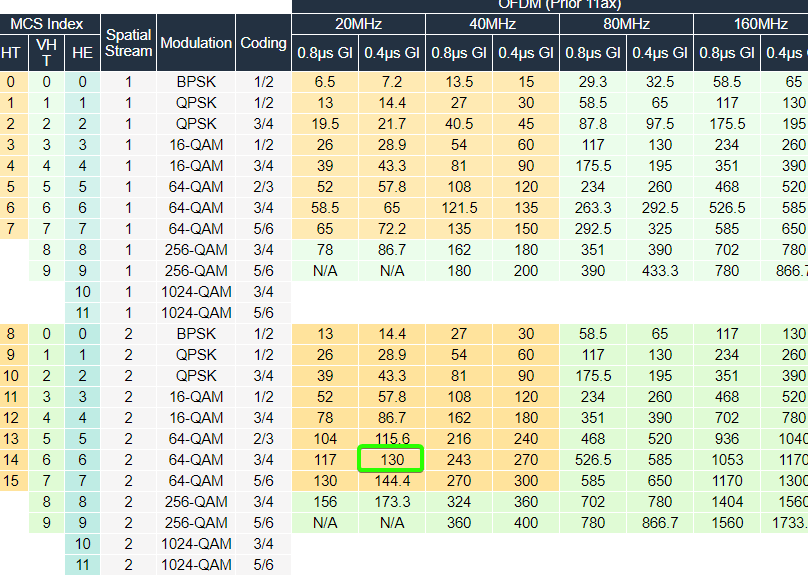
\includegraphics[width=0.8
    \linewidth]{src/chrome_GUtrJRqsad.png}
    \caption{\label{fig:mcsindex} Modulación elegida.}
\end{figure}
\newpage
Se elige 64-QAM 3/4. Viendo el \textbf{datasheet}, la antena receptora tendrá una sensibilidad de -77dBm y margen de 2. (CAMBIAR)

\subsection{RadioMobile}

\subsection{Resultados de los radioenlaces}

\section{Diseño de la Red}

\section{Conclusión?}


\end{document}